% !TeX root = aaai2027.tex
% !TeX encoding = UTF-8
% !TeX program = pdflatex
% !BIB program = bibtex
\documentclass[letterpaper]{article} % DO NOT CHANGE THIS
\usepackage[submission]{aaai2027}  % DO NOT CHANGE THIS
% The serif, sans-serif, and monospaced fonts are loaded automatically by
% aaai2027.sty (newtxtext, helvet, courier). DO NOT add \usepackage{times},
% \usepackage{helvet}, \usepackage{courier}, or any other font package.
\usepackage[hyphens]{url}  % DO NOT CHANGE THIS
\usepackage{graphicx} % DO NOT CHANGE THIS
\urlstyle{rm} % DO NOT CHANGE THIS
\def\UrlFont{\rm}  % DO NOT CHANGE THIS
\usepackage{natbib}  % DO NOT CHANGE THIS AND DO NOT ADD ANY OPTIONS TO IT
\usepackage{caption} % DO NOT CHANGE THIS AND DO NOT ADD ANY OPTIONS TO IT
\frenchspacing  % DO NOT CHANGE THIS
%
% These are recommended to typeset algorithms but not required. See the subsubsection on algorithms. Remove them if you don't have algorithms in your paper.
\usepackage{algorithm}
\usepackage{algorithmic}
\usepackage{graphicx}
%
% These are recommended to typeset listings but not required. See the subsubsection on listing. Remove this block if you don't have listings in your paper.
\usepackage{newfloat}
\usepackage{listings}


\DeclareCaptionStyle{ruled}{labelfont=normalfont,labelsep=colon,strut=off} % DO NOT CHANGE THIS
\lstset{%
	basicstyle={\footnotesize\ttfamily},% footnotesize acceptable for monospace
	numbers=left,numberstyle=\footnotesize,xleftmargin=2em,% show line numbers, remove this entire line if you don't want the numbers.
	aboveskip=0pt,belowskip=0pt,%
	showstringspaces=false,tabsize=2,breaklines=true}
\floatstyle{ruled}
\newfloat{listing}{tb}{lst}{}
\floatname{listing}{Listing}

%
% Recommended for better-looking tables
\usepackage{booktabs}

%
% Keep the \pdfinfo as shown here. There's no need
% for you to add the /Title and /Author tags.
\pdfinfo{
/TemplateVersion (2027.1)
}

% DISALLOWED PACKAGES
% \usepackage{authblk} -- This package is specifically forbidden
% \usepackage{balance} -- This package is specifically forbidden
% \usepackage{CJK} -- This package is specifically forbidden
% \usepackage{float} -- This package is specifically forbidden
% \usepackage{flushend} -- This package is specifically forbidden
% \usepackage{fullpage} -- This package is specifically forbidden
% \usepackage{geometry} -- This package is specifically forbidden
% \usepackage{hyperref} -- This package is specifically forbidden
% \usepackage{navigator} -- This package is specifically forbidden
% (or any other package that embeds links such as navigator or hyperref)
% \usepackage{indentfirst} -- This package is specifically forbidden
% \usepackage{layout} -- This package is specifically forbidden
% \usepackage{multicol} -- This package is specifically forbidden
% \usepackage{nameref} -- This package is specifically forbidden
% \usepackage{savetrees} -- This package is specifically forbidden
% \usepackage{setspace} -- This package is specifically forbidden
% \usepackage{stfloats} -- This package is specifically forbidden
% \usepackage{tabu} -- This package is specifically forbidden
% \usepackage{titlesec} -- This package is specifically forbidden
% \usepackage{tocbibind} -- This package is specifically forbidden
% \usepackage{ulem} -- This package is specifically forbidden
% \usepackage{wrapfig} -- This package is specifically forbidden
% DISALLOWED COMMANDS
% \nocopyright -- Your paper will not be published if you use this command
% \addtolength -- This command may not be used
% \balance -- This command may not be used
% \baselinestretch -- Your paper will not be published if you use this command
% \clearpage -- No page breaks of any kind may be used for the final version of your paper
% \columnsep -- This command may not be used
% \newpage -- No page breaks of any kind may be used for the final version of your paper
% \pagebreak -- No page breaks of any kind may be used for the final version of your paper
% \pagestyle -- This command may not be used
% \tiny -- This is not an acceptable font size.
% \vspace{- -- No negative value may be used in proximity of a caption, figure, table, section, subsection, subsubsection, or reference
% \vskip{- -- No negative value may be used to alter spacing above or below a caption, figure, table, section, subsection, subsubsection, or reference

\setcounter{secnumdepth}{0} %May be changed to 1 or 2 if section numbers are desired.

% The file aaai2027.sty is the style file for AAAI Press
% proceedings, working notes, and technical reports.
%

% Title

% Your title must be in mixed case, not sentence case.
% That means all verbs (including short verbs like be, is, using,and go),
% nouns, adverbs, adjectives should be capitalized, including both words in hyphenated terms, while
% articles, conjunctions, and prepositions are lower case unless they
% directly follow a colon or long dash
\title{TLDR: Token-Level Late-interaction for Direct hotword Retrieval}
\author{
    %Authors
    % All authors must be in the same font size and format.
    Written by AAAI Press Staff\textsuperscript{\rm 1}\thanks{With help from the AAAI Publications Committee.}\\
    AAAI Style Contributions by Peter Patel Schneider,
    Sunil Issar,\\
    J. Scott Penberthy,
    George Ferguson,
    Hans Guesgen,
    Francisco Cruz\equalcontrib\corresponding,
    Marc Pujol-Gonzalez\equalcontrib\corresponding
    }
\affiliations{
    %Afiliations
    \textsuperscript{\rm 1}Association for the Advancement of Artificial Intelligence\\
    % If you have multiple authors and multiple affiliations
    % use superscripts in text and roman font to identify them.
    % For example,

    % Sunil Issar\textsuperscript{\rm 2},
    % J. Scott Penberthy\textsuperscript{\rm 3},
    % George Ferguson\textsuperscript{\rm 4}\corresponding,
    % Hans Guesgen\textsuperscript{\rm 5}
    % Note that the comma should be placed after the superscript

    1101 Pennsylvania Ave, NW Suite 300\\
    Washington, DC 20004 USA\\
    % email address must be in roman text type, not monospace or sans serif
    proceedings-questions@aaai.org
%
% See more examples next
}

%Example, Single Author, ->> remove \iffalse,\fi and place them surrounding AAAI title to use it
\iffalse
\title{My Publication Title --- Single Author}
\author {
    Author Name
}
\affiliations{
    Affiliation\\
    Affiliation Line 2\\
    name@example.com
}
\fi

\iffalse
%Example, Multiple Authors, ->> remove \iffalse,\fi and place them surrounding AAAI title to use it
\title{My Publication Title --- Multiple Authors}
\author {
    % Authors
    First Author Name\textsuperscript{\rm 1,\rm 2}\equalcontrib,
    Second Author Name\textsuperscript{\rm 2}\equalcontrib,
    Third Author Name\textsuperscript{\rm 1}\corresponding
}
\affiliations {
    % Affiliations
    \textsuperscript{\rm 1}Affiliation 1\\
    \textsuperscript{\rm 2}Affiliation 2\\
    firstAuthor@affiliation1.com, secondAuthor@affilation2.com, thirdAuthor@affiliation1.com
}
\fi


\begin{document}

\maketitle

\begin{abstract}
AAAI creates proceedings, working notes, and technical reports directly from electronic source furnished by the authors. To ensure that all papers in the publication have a uniform appearance, authors must adhere to the following instructions.
\end{abstract}

% Uncomment the following to link to your code, datasets, an extended version or similar.
% You must keep this block between (not within) the abstract and the main body of the paper.
% Make sure that you do not de-anonymize yourself with these links.
% \begin{links}
%     \link{Code}{https://aaai.org/example/code}
%     \link{Datasets}{https://aaai.org/example/datasets}
%     \link{Extended version}{https://aaai.org/example/extended-version}
% \end{links}

\section{Introduction}

Speech large language models and prompt-based automatic speech recognition (ASR) systems have substantially improved the flexibility of speech understanding. By conditioning recognition on textual prompts or task instructions, these systems can exploit strong internal language priors and adapt to diverse user contexts. However, the same priors also make them vulnerable when recognizing named entities, rare words, and other long-tail expressions. Such words are sparse in training data, often acoustically ambiguous, and may differ from frequent alternatives by only a few phonetic units. As a result, ASR errors on these terms commonly appear as substitutions into high-frequency words, semantically plausible phrases, or similarly pronounced entities.

Retrieval-augmented contextual ASR provides a practical way to address this limitation. Instead of modifying the main ASR model, a retriever selects candidate hotwords from an external vocabulary or contextual source, and the selected candidates are injected into the ASR prompt as biasing context. This paradigm is attractive because it can improve recognition of domain-specific entities while keeping the recognizer fixed. Recent contrastive hotword retrievers have shown the potential of this direction \cite{kong25_interspeech}. Nevertheless, contextual ASR is only as reliable as the retrieved candidates: missing the true entity limits the benefit of prompting, while retrieving confusable false positives may further bias the recognizer toward incorrect words.

Existing speech-text retrieval methods face two challenges in this setting. First, \emph{representation dilution} occurs when a long utterance is compressed into a single global embedding. Since hotwords are often short spans, their acoustic evidence can be overwhelmed by surrounding speech content, especially for entity-rich utterances. Second, \emph{alignment drift under weak supervision} arises when timestamp annotations are unavailable. With only utterance-level transcripts and hotword labels, a model may learn broad sentence-level semantic association rather than the local acoustic-text correspondence needed to determine whether a specific candidate was actually spoken. These two issues make global retrieval objectives poorly matched to fine-grained hotword search.

\begin{figure}[t]
  \centering
  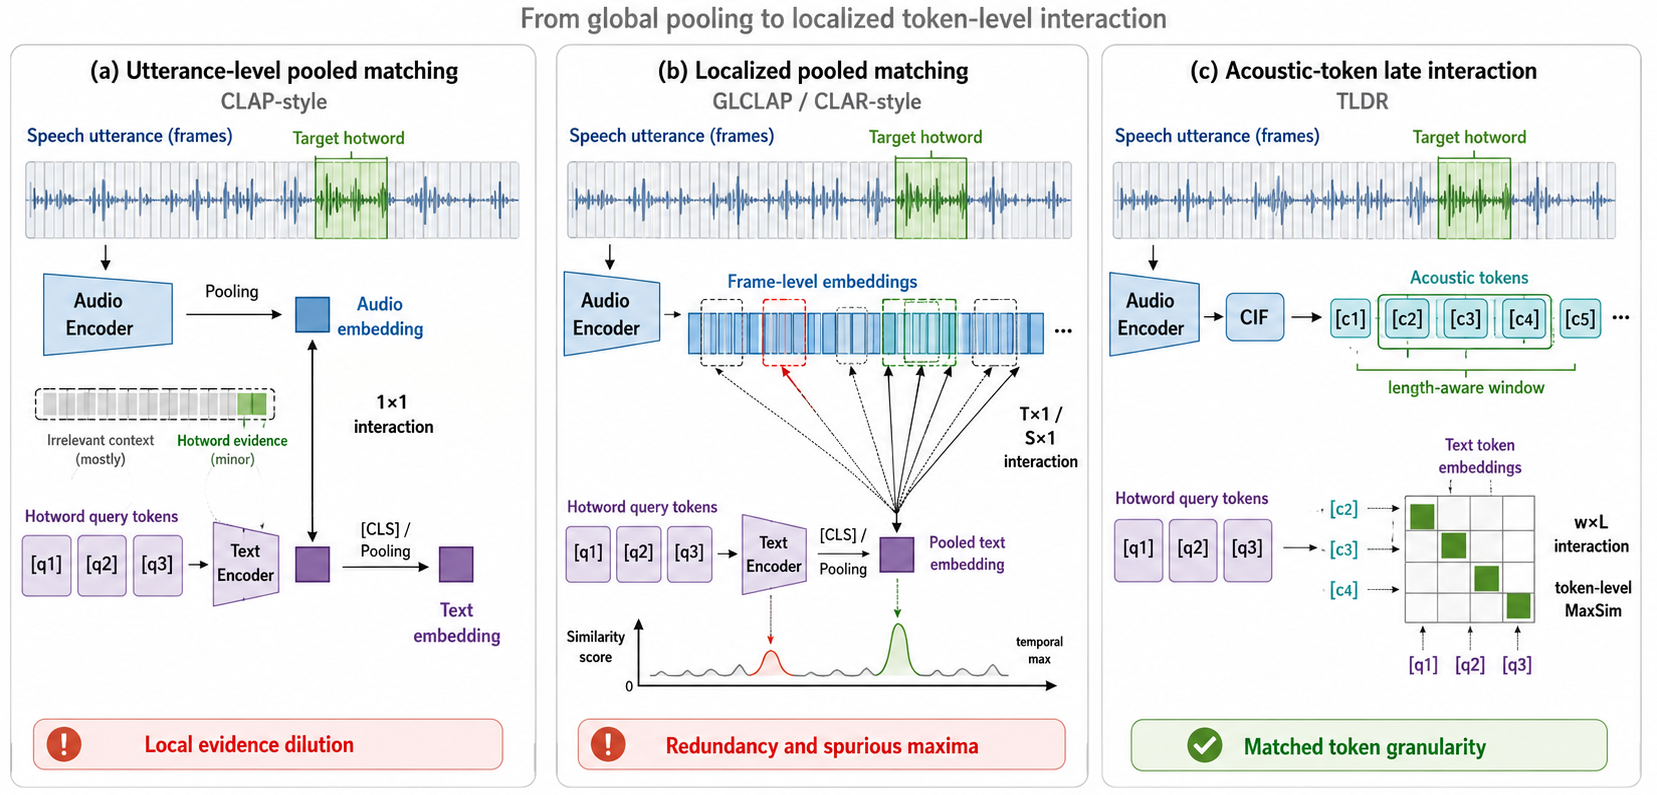
\includegraphics[width=1\linewidth]{figure/intro.png}
  \caption{Comparison of hotword retrieval paradigms. (a) Existing retrievers compress long speech into global embeddings or unconstrained local features, where short hotword cues are diluted or suffer from alignment drift. (b) Our method tokenizes speech into monotonic acoustic tokens via CIF and performs length-aware local late interaction to preserve fine-grained entity details under weak supervision.}
  \label{fig:intro}
\end{figure}

We propose TLDR, a acoustic-text retriever for retrieval-augmented contextual ASR. As illustrated in Figure~\ref{fig:intro}, TLDR first converts continuous speech frames into a monotonic acoustic-token sequence using continuous integrate-and-fire (CIF). It then slides a candidate-length window over the acoustic tokens and applies token-level Text MaxSim as a late-interaction scoring function. This design keeps the retrieval decision localized while remaining robust to small boundary errors. We train the retriever with local contrastive learning, CIF quantity regularization, and an auxiliary token-level alignment objective, together with false-negative-aware batch construction for reliable in-batch contrastive learning.

Our contributions are summarized as follows:
\begin{itemize}
\item We formulate hotword retrieval for contextual ASR as a weakly supervised localized cross-modal retrieval problem, where short textual entities must be matched against long speech utterances without timestamp annotations.
\item We propose a CIF-guided acoustic-token late-interaction retriever. It converts continuous speech into monotonic acoustic tokens and performs length-aware Text MaxSim matching over local windows, preserving fine-grained entity cues without explicit temporal labels.
\item We introduce reliable contrastive training strategies, including CIF quantity regularization, token-level auxiliary alignment, and false-negative-aware batch construction, targeting strong hotword retrieval and downstream contextual ASR improvements.
\end{itemize}

\begin{figure*}[ht]
  \centering
  
\includegraphics[width=0.8\textwidth]{figure/method.png}
  \caption{TLDR, a CIF-guided local acoustic-text retrieval framework for spoken hotword retrieval.}
  \label{fig:method}
\end{figure*}

\section{Related Work}

\subsection{Audio-Text Contrastive Retrieval}

Audio-text contrastive learning provides a natural framework for transcription-free speech-text retrieval by aligning acoustic inputs and textual descriptions in a shared embedding space. However, most CLAP-style retrievers operate at utterance or phrase level, which is insufficient for hotword retrieval where the relevant evidence often occupies only a short local span. Recent localized retrievers such as GLCLAP~\cite{kong25_interspeech} and CLAR~\cite{huang2026clar} mitigate this issue by introducing local acoustic-text matching. Nevertheless, their scoring functions still largely compare local acoustic regions with phrase-level candidate representations, which may obscure token-level distinctions among short, phonetically similar, or substring-related hotwords. TLDR addresses this gap by preserving candidate hotwords as token sequences and performing token-level late interaction with localized acoustic tokens.

\subsection{Contextual Biasing and Hotword Retrieval}

Contextual biasing improves ASR recognition of rare words, named entities, and domain-specific phrases by incorporating external bias phrases into the recognizer. Existing methods mainly study how to inject or utilize a given bias list during decoding or representation learning. In contrast, our work focuses on a preceding retrieval problem: when the candidate list is large and noisy, the system must first identify which hotwords are acoustically supported by the input speech. TLDR is therefore complementary to contextual biasing methods, providing a compact and more reliable hotword set before downstream bias injection.

\subsection{Acoustic Tokenization and Late Interaction}

CIF converts dense frame-level speech representations into monotonic token-like acoustic units, reducing the granularity mismatch between acoustic frames and text tokens. This makes it suitable for localized hotword retrieval, where short text queries should be matched against compact acoustic spans. TLDR is also inspired by late-interaction retrieval, which preserves token-level representations and computes fine-grained matching at scoring time. Unlike text retrieval, speech-hotword retrieval requires temporal compactness and monotonicity. TLDR therefore combines CIF-based acoustic tokenization, length-aware local windows, and token-level late interaction for fine-grained transcription-free hotword retrieval.


\section{Method}

We propose TLDR, a CIF-guided local acoustic-text retrieval framework for spoken hotword retrieval. Given a speech utterance and a set of candidate hotwords, TLDR directly scores each candidate against acoustic evidence from the utterance, instead of first producing a complete ASR transcript and then applying text matching. The central design is to convert continuous frame-level speech representations into monotonic acoustic tokens with continuous integrate-and-fire (CIF), and then perform length-aware local matching between candidate hotword tokens and sliding acoustic-token windows.

\subsection{Task Formulation}

Let $x$ denote an input speech utterance and let $\mathcal{H}=\{h_1,\ldots,h_N\}$ be a candidate hotword set. The model computes a relevance score for each candidate,
\begin{equation}
s(x,h_i), \quad i=1,\ldots,N,
\end{equation}
and returns either a ranked list of candidates or a predicted hotword set by thresholding the scores. During training, each example contains the utterance, its full transcript, and one or more annotated hotwords. The transcript is used to construct token-level supervision and to regularize acoustic tokenization, but at inference time TLDR only requires the speech utterance and the candidate hotword set.

This formulation differs from utterance-level speech-text retrieval. A hotword is often a short span inside a much longer utterance, so an utterance-level embedding may dilute the local acoustic evidence. TLDR therefore treats spoken hotword retrieval as local evidence search: a candidate should receive a high score only if it is supported by some local acoustic-token region in the utterance.

\subsection{Model Overview}



Figure~\ref{fig:method}  TLDR follows a dual-encoder design with an acoustic encoder, a text encoder, projection heads, and a CIF-based acoustic tokenizer. The acoustic encoder maps input speech or acoustic features into frame-level hidden states
\begin{equation}
H^a=[h^a_1,\ldots,h^a_T], \quad h^a_t \in \mathbf{R}^{d_a}.
\end{equation}
A two-layer projection head maps the frame representations into a shared retrieval space and applies L2 normalization,
\begin{equation}
z^a_t = \frac{g_a(h^a_t)}{\|g_a(h^a_t)\|_2}.
\end{equation}
The text encoder maps both full transcripts and hotword candidates into token-level hidden states. For a candidate hotword $h_i$ with $L_i$ content tokens, the projected and normalized token embeddings are
\begin{equation}
Q_i=[q_{i,1},\ldots,q_{i,L_i}], \quad q_{i,l} \in \mathbf{R}^{d}.
\end{equation}
Keeping token-level candidate representations is important because the retrieval score is computed from local token matches rather than a single pooled text embedding.

\subsection{CIF-Guided Acoustic Tokenization}

Directly matching text tokens to frame-level speech representations is inefficient and unstable because speech frames are much longer and have a different granularity from text tokens. TLDR therefore uses CIF to compress frame-level acoustic representations into a shorter sequence of acoustic tokens.

For each frame, a CIF predictor estimates a non-negative weight $\alpha_t$. The weights are accumulated from left to right. When the accumulated mass reaches a firing threshold $\theta$, the model emits one acoustic token by aggregating the corresponding frame representations:
\begin{equation}
c_j = \mathrm{CIF}(Z^a,\alpha)_j.
\end{equation}
This yields an acoustic-token sequence
\begin{equation}
C=[c_1,\ldots,c_M],
\end{equation}
where the order of tokens preserves the monotonic temporal structure of speech.

During training, we regularize the number of emitted acoustic tokens with a quantity loss:
\begin{equation}
\mathcal{L}_{\mathrm{cif}} =
\left| \sum_{t=1}^{T} \alpha_t - L_{\mathrm{text}} \right|.
\end{equation}
Here $L_{\mathrm{text}}$ is the transcript token length. This constraint encourages the acoustic tokenizer to emit a sequence whose length is compatible with text-token matching. As a result, downstream local matching operates on acoustic tokens rather than raw frames, reducing both sequence length and granularity mismatch.

\subsection{Length-Aware Local Hotword Matching}

For a candidate hotword $h_i$, TLDR constructs sliding windows over the CIF acoustic-token sequence. The window length is set to the number of candidate text tokens $L_i$:
\begin{equation}
W_{s,i}=[c_s,\ldots,c_{s+L_i-1}],
\quad s=1,\ldots,M-L_i+1.
\end{equation}
Each window is scored against the candidate with token-level Text MaxSim. Since both acoustic and text embeddings are normalized, dot products correspond to cosine similarities:
\begin{equation}
m(W_{s,i},h_i)=
\frac{1}{L_i}
\sum_{l=1}^{L_i}
\max_{c \in W_{s,i}} c^\top q_{i,l}.
\end{equation}
The final local retrieval score is the best-matching window score:
\begin{equation}
s_{\mathrm{local}}(x,h_i)=
\max_s m(W_{s,i},h_i).
\end{equation}

This matching function is length-aware because each candidate determines its own window size. It is also tolerant to small CIF boundary errors: a text token only needs to find a strong match inside the local acoustic window, rather than being forced into a strict one-to-one alignment. The outer maximization over windows lets the model jointly localize and retrieve the hotword inside the full utterance.

\subsection{Training Objectives}

The primary retrieval objective is a local contrastive loss over in-batch speech-hotword pairs. For a batch of $B$ paired examples, we compute a similarity matrix $S \in \mathbf{R}^{B \times B}$ using local MaxSim scores, where $S_{b,j}=s_{\mathrm{local}}(x_b,h_j)$. The diagonal entries are positives and off-diagonal entries are in-batch negatives. We optimize a bidirectional contrastive loss:
\begin{equation}
\mathcal{L}_{a2t}
=-\frac{1}{B}\sum_{b=1}^{B}
\log
\frac{\exp(S_{b,b}/\tau)}
{\sum_{j=1}^{B}\exp(S_{b,j}/\tau)},
\end{equation}
\begin{equation}
\mathcal{L}_{t2a}
=-\frac{1}{B}\sum_{b=1}^{B}
\log
\frac{\exp(S_{b,b}/\tau)}
{\sum_{j=1}^{B}\exp(S_{j,b}/\tau)},
\end{equation}
\begin{equation}
\mathcal{L}_{\mathrm{local}}
=\frac{1}{2}\mathcal{L}_{a2t}
+\frac{1}{2}\mathcal{L}_{t2a}.
\end{equation}

In addition to the local retrieval objective and CIF quantity loss, TLDR uses a token-level auxiliary objective over full utterances. The auxiliary branch aligns the CIF acoustic-token sequence with the full transcript token sequence using index-aligned token-level contrastive learning. This branch is not treated as the main hotword ranking signal; instead, it regularizes the shared embedding space and stabilizes token-level acoustic-text representations.

The overall training objective is
\begin{equation}
\mathcal{L}
= \lambda_{\mathrm{local}}\mathcal{L}_{\mathrm{local}}
+ \lambda_{\mathrm{cif}}\mathcal{L}_{\mathrm{cif}}
+ \lambda_{\mathrm{gu}}\mathcal{L}_{\mathrm{gu}}.
\end{equation}
An optional utterance-level global contrastive loss can also be used as a weak regularizer, but TLDR's core retrieval behavior comes from the local MaxSim branch. This distinction is important because utterance-level global matching optimizes coarse speech-text similarity, while hotword retrieval requires local evidence for a short candidate span.

\subsection{False-Negative Aware Batch Construction}

In-batch contrastive learning assumes that off-diagonal pairs are true negatives. This assumption can be violated in hotword retrieval: two utterances may share a hotword, or a hotword from one example may appear in another example's transcript. Treating such pairs as negatives would push apart valid acoustic-text matches.

We therefore construct training batches with false-negative filtering. A pair of examples is not used as mutual negatives if their hotword sets overlap, if a hotword from the first example appears in the second transcript, or if a hotword from the second example appears in the first transcript. This filtering makes the local contrastive objective better aligned with the multi-hotword nature of the task.

\subsection{Inference}

At inference time, candidate hotword embeddings can be precomputed once with the text encoder. For each input utterance, TLDR extracts CIF acoustic tokens and computes $s_{\mathrm{local}}(x,h_i)$ for every candidate. The final score can optionally combine the local score with weak auxiliary scores:
\begin{equation}
\begin{array}{l}
s(x,h_i)=w_{\mathrm{local}}s_{\mathrm{local}}(x,h_i) \\
\quad + w_{\mathrm{gu}}s_{\mathrm{gu}}(x,h_i) \\
\quad + w_{\mathrm{global}}s_{\mathrm{global}}(x,h_i).
\end{array}
\end{equation}
In the main retrieval setting, $w_{\mathrm{local}}$ is the dominant weight, while the global and token-level auxiliary scores are either disabled or used with small weights for calibration. The predicted hotword set is then obtained by ranking candidates or applying a decision threshold to the final scores.

\newpage
\bibliography{aaai2027}

% Check whether the conference requires a reproducibility checklist to be included in the paper.
% If so, you can uncomment the following line and ajust the path to include it.
% \input{ReproducibilityChecklist.tex}

\end{document}
